% CVPR 2026 Paper Template

\documentclass[10pt,twocolumn,letterpaper]{article}

\usepackage[pagenumbers]{cvpr}

% Import additional packages in the preamble file, before hyperref
%% This file contains a number of tweaks that are typically applied to the main document.

\usepackage[utf8]{inputenc}
\usepackage[T1]{fontenc}
\usepackage{booktabs}
\usepackage{multirow}
\usepackage{amsmath}
\graphicspath{{../results/}{../results/domain_adaptation/}}

%%
%% Inline annotations
%%
\newcommand{\red}[1]{{\color{red}#1}}
\newcommand{\todo}[1]{{\color{red}#1}}
\newcommand{\TODO}[1]{\textbf{\color{red}[TODO: #1]}}
%%
%% disable for camera ready / submission by uncommenting these lines  
%%
% \renewcommand{\TODO}[1]{}
% \renewcommand{\todo}[1]{#1}

%%
%% work harder in optimizing text layout. Typically shrinks text by 1/6 of page, enable
%% it at the very end of the writing process, when you are just above the page limit
%%
% \usepackage{microtype}

%%
%% fine-tune paragraph spacing
%%
% \renewcommand{\paragraph}[1]{\vspace{.5em}\noindent\textbf{#1.}}

%%
%% globally adjusts space between figure and caption
%%
% \setlength{\abovecaptionskip}{.5em}


%%
%% Allows "the use of \paper to refer to the project name"
%% with automatic management of space at the end of the word
%%
% \usepackage{xspace}
% \newcommand{\paper}{ProjectName\xspace}

%%
%% Commonly used math definitions
%%
% \DeclareMathOperator*{\argmin}{arg\,min}
% \DeclareMathOperator*{\argmax}{arg\,max}

%%
%% Tigthen underline
%%
% \usepackage{soul}
% \setuldepth{foobar}

\definecolor{cvprblue}{rgb}{0.21,0.49,0.74}
\usepackage[pagebackref,breaklinks,colorlinks,allcolors=cvprblue]{hyperref}

\def\paperID{*****}
\def\confName{CVPR}
\def\confYear{2026}

\title{Ré-identification de Personnes~: Approches Classiques,\\
Apprentissage Profond et Adaptation de Domaine}

\author{
Daphné Maschas \quad Adham Noureldin \quad Maxence Rossignol \\
CentraleSupélec, Université Paris-Saclay \\
{\tt\small \{daphne.maschas, adham.noureldin, maxence.rossignol\}@student-cs.fr}
}

\begin{document}
\maketitle
\begin{abstract}
Ce travail présente une étude experimentale de la ré-identification de personnes (Re-ID) à travers sept contributions couvrant l'intégralité de la chaine, du prétraitement à l'indexation d'albums sans supervision. Nous évaluons nos approches sur Market-1501 (32\,668 images, 1,501 identités, 6 caméras) et sur un jeu de données personnel collecté via une pipeline de détection YOLOv8n. Dans un premier temps, nous confrontons des descripteurs classiques de vision par ordinateur (HOG, histogramme de couleur, SIFT) à un modèle profond ResNet-50 entraîné avec une perte combinée identitaire et triplet: l'écart est considérable, avec un Rank-1 passant de 0,68\,\% \`{a} 84,41\,\% en faveur de l'apprentissage profond. Une étude d'ablation sur les stratégies de gel du réseau révele que le fine-tuning complet surpasse nettement le gel total du backbone (85,36\,\% vs 7,07\,\% en Rank-1). La comparaison CNN/Transformer indique que ViT-Base/16 dépasse ResNet-50 en Rank-1 (88,63\,\% vs 84,41\,\%) et en mAP (73,84\,\% vs 64,47\,\%), au coût d'un budget paramétrique 3,45$\times$ plus élevé. L'adaptation de domaine de Market-1501 vers un jeu de données personnel montre une amélioration de la mAP de 78,27\,\% \`{a} 89,93\,\% grâce au transfer learning. Enfin, le clustering DBSCAN sur les embeddings ResNet-50 permet une indexation automatique d'albums avec une pureté de 88,95\,\% sur Market-1501 et 94,80\,\% sur le dataset personnel.
\end{abstract}
\section{Introduction}
\label{sec:intro}

La ré-identification de personnes (Re-ID) est la t\^{a}che de retrouver une personne d'intérêt dans un large ensemble d'images provenant de caméras non articulées, à des moments et des points de vue différents. Dans un système de surveillance multi-caméras, une même personne peut apparaître très différemment selon l'angle de prise de vue, les conditions d'éclairage ou son habillement : construire un descripteur robuste à ces variations est l'enjeu central du Re-ID.

Les applications sont nombreuses : sécurité et surveillance en espace public, assistance aux personnes vulnérables, analyse du flux de visiteurs dans le commerce de détail, ou encore investigations médico-légales. Ces contextes partagent une contrainte commune : le système doit fonctionner sous de fortes variations intra-classe (même personne vue différemment) tout en séparant clairement les classes inter-identités.

\paragraph{Défis.}
Les principaux obstacles à un Re-ID fiable sont : (i) les variations d'illumination entre intérieur et extérieur ; (ii) les occultations partielles par des obstacles ou d'autres personnes ; (iii) les changements de pose et de point de vue ; (iv) la variabilité intra-classe (même vêtement sous éclairages différents), et (v) le gap de domaine entre jeu de données d'entraînement (Market-1501) et scène réelle.

\paragraph{Contributions.}
Ce rapport présente sept contributions expérimentales (\textbf{WP1--WP7}) couvrant la chaîne complète :
\begin{enumerate}
\item \textbf{WP1} : Impact systématique du prétraitement (résolution, espace de couleur, filtres, augmentation) sur les performances de Re-ID.
\item \textbf{WP2} : Comparaison rigoureuse des descripteurs classiques (HOG, histogramme de couleur, SIFT) face aux embeddings profonds avec et sans re-ranking.
\item \textbf{WP3} : Constitution d'un jeu de données personnel via un pipeline de détection automatique YOLOv8.
\item \textbf{WP4} : Ablation sur trois stratégies de gel du réseau (feature extraction, fine-tuning partiel, fine-tuning complet).
\item \textbf{WP5} : Comparaison CNN/Transformer au sens du Rank-1, mAP, co\^{u}t paramétrique et latence d'inférence.
\item \textbf{WP6} : Adaptation de domaine de Market-1501 vers le dataset personnel par zero-shot et transfer learning.
\item \textbf{WP7} : Indexation automatique d'albums par clustering DBSCAN sur les embeddings appris.
\end{enumerate}

\section{Définition du problème}
\label{sec:problem}

\paragraph{Notation.}
Soit $\mathcal{G} = \{(\mathbf{x}_i, y_i)\}_{i=1}^{N_G}$ la galerie d'images annotées avec des identités $y_i \in \{1, \ldots, P\}$, et soit $\mathbf{q}$ une image requête d'identité $y_q$ a priori inconnue dans $\mathcal{G}$. L'objectif est d'ordonner les images de $\mathcal{G}$ par ordre croissant de distance à $\mathbf{q}$ :
\begin{equation}
\pi^* = \operatorname{argsort}_{i=1}^{N_G} \; d\!\left(f_\theta(\mathbf{q}),\, f_\theta(\mathbf{x}_i)\right)
\label{eq:ranking}
\end{equation}
o\`{u} $f_\theta : \mathbb{R}^{H \times W \times 3} \to \mathbb{R}^d$ est le réseau extracteur d'embeddings et $d(\mathbf{a}, \mathbf{b}) = \|\mathbf{a} - \mathbf{b}\|_2$ la distance euclidienne. Conformément au protocole standard \cite{zheng2015scalable}, les paires (requête, galerie) provenant du même angle de caméra et de la même séquence sont exclues de l'évaluation.

\paragraph{Fonction objectif.}
Le réseau est optimisé par minimisation d'une perte combinée :
\begin{equation}
\mathcal{L} = \mathcal{L}_{\text{CE}}(f_\theta) + \mathcal{L}_{\text{tri}}(f_\theta)
\label{eq:loss_total}
\end{equation}
La perte identitaire $\mathcal{L}_{\text{CE}}$ est une entropie croisée softmax sur les $P$ classes d'identité. La perte triplet avec minage difficile (\textit{hard mining}) \cite{hermans2017defense} est calculée pour chaque ancre $\mathbf{x}_a$ dans le batch :
\begin{equation}
\begin{split}
\mathcal{L}_{\text{tri}} &= \frac{1}{B}\!\sum_{a=1}^{B}\!\bigg[\,m + \underbrace{\max_{j:\,y_j = y_a}\!d(f(\mathbf{x}_a), f(\mathbf{x}_j))}_{\text{positif le plus difficile}} \\
&\quad - \underbrace{\min_{k:\,y_k \neq y_a}\!d(f(\mathbf{x}_a), f(\mathbf{x}_k))}_{\text{négatif le plus difficile}}\,\bigg]_+
\end{split}
\label{eq:triplet}
\end{equation}
avec marge $m = 0{,}3$ et $[\,\cdot\,]_+ = \max(0, \cdot)$.

\paragraph{Métriques d'évaluation.}
La précision \textbf{Rank-$k$} (CMC\,@$k$) mesure la fraction des requêtes pour lesquelles au moins une correspondance correcte figure dans les $k$ premières propositions. La \textbf{mAP} (\textit{mean Average Precision}) évalue la qualité globale du classement en agrégeant la précision à chaque rang de récupération :
\begin{equation}
\text{mAP} = \frac{1}{|\mathcal{Q}|}\sum_{\mathbf{q} \in \mathcal{Q}} \frac{\displaystyle\sum_{k=1}^{N_G} P(k)\cdot\mathbf{1}[y_{\pi(k)} = y_q]}{|\{i : y_i = y_q\}|}
\label{eq:map}
\end{equation}
La mAP est plus discriminante que le Rank-1 lorsque plusieurs images de la même personne sont présentes dans la galerie.

%-------------------------------------------------------------------------

\section{Travaux connexes}
\label{sec:related}

\paragraph{Jeux de données de référence.}
Market-1501~\cite{zheng2015scalable} est le benchmark standard de Re-ID en milieu contrôl é: 32,668 images de 1,501 identités captur ées par 6 caméras sur le campus de l'Université Tsinghua. Sa pertinence réside dans la diversité des points de vue et dans un protocole d'évaluation bien défini (exclusion des paires même caméra, CMC, mAP). Ce benchmark reste la référence pour la comparaison des approches modernes~\cite{ye2021deep}.

\paragraph{Descripteurs classiques.}
Avant l'ère de l'apprentissage profond, les approches Re-ID s'appuyaient sur des descripteurs à la main. Les histogrammes de gradients orientés (HOG)~\cite{dalal2005histograms} et les \textit{Scale-Invariant Feature Transform} (SIFT)~\cite{lowe2004distinctive} capturent respectivement la texture et les points saillants locaux. Ces descripteurs souffrent de la sensibilité aux changements d'éclairage et de point de vue, ce qui limite leurs performances en Re-ID.

\paragraph{Apprentissage profond pour le Re-ID.}
Depuis l'avènement des réseaux de neurones convolutifs, les approches profondes dominent le domaine~\cite{ye2021deep}. La \og{}Bag of Tricks\fg{} (BoT)~\cite{luo2019bag} a établi une base solide en introduisant le \textit{BN-Neck} (BatchNorm entre l'extracteur et le classifieur), l'astuce \textit{last\_stride=1} pour conserver la résolution spatiale, et la perte triplet combinée à l'entropie croisée~-- notre architecture s'en inspire directement.

\paragraph{Transformers pour le Re-ID.}
TransReID~\cite{he2021transreid} est l'une des premières approches à adapter les Vision Transformers (ViT)~\cite{dosovitskiy2021image} au Re-ID. En exploitant le mécanisme d'attention globale, ces modèles capturent des dépendances longue portée que les CNN peinent à modéliser, au prix d'un co\^{u}t de calcul plus élevé.

\paragraph{Apprentissage de métriques.}
La perte triplet avec minage difficile, formalisée par Hermans \textit{et al.}~\cite{hermans2017defense}, est devenue le standard pour l'apprentissage de représentations discriminantes en Re-ID. Elle force le réseau à rapprocher les exemples de même identité et à séparer les négatifs les plus proches.

\paragraph{Re-ranking.}
Zhong \textit{et al.}~\cite{zhong2017re} proposent une procédure de re-classement basée sur l'encodage k-réciproque, qui raffine la matrice de distance initiale en tenant compte des voisins mutuels~-- une technique post-traitement efficace qui peut gagner plusieurs points de mAP sans modifier le modèle.

\paragraph{Clustering sans supervision.}
DBSCAN~\cite{ester1996density} est un algorithme de clustering basé sur la densité qui ne nécessite pas de préciser le nombre de clusters \textit{a~priori}~-- un avantage considérable pour l'indexation d'albums o\`{u} le nombre d'identités est inconnu.

\section{Méthodologie}
\label{sec:methodology}

\subsection{Vue d'ensemble du pipeline}

Notre pipeline complet comprend quatre étapes : (1) constitution du jeu de données (détection YOLO pour le dataset personnel), (2) prétraitement et augmentation, (3) extraction d'embeddings par un réseau Re-ID, et (4) évaluation par CMC/mAP avec re-ranking optionnel. Pour le clustering (WP7), l'étape 4 est remplacée par un regroupement DBSCAN.

\subsection{Jeux de données}

\paragraph{Market-1501.}
Market-1501 \cite{zheng2015scalable} comprend 32\,668 images de 1\,501 identités capturées par 6 caméras. La partition standard définit 12\,936 images d'entraînement (751 identités), 3\,368 requêtes et 13\,115 images de galerie (750 identités). La résolution des images varie selon la caméra ; toutes sont redimensionnées à $256 \times 128$ px.

\paragraph{Dataset personnel (WP3).}
Pour étudier l'adaptation de domaine, nous avons constitué un jeu de données personnel de 262 images capturées sur le campus de CentraleSupélec. La détection automatique des personnes est réalisée par \textbf{YOLOv8n} \cite{ultralytics2023}, un détecteur léger (\textit{nano}) de la famille Ultralytics YOLO, qui recadre automatiquement chaque personne détectée. Les annotations d'identité (pour l'évaluation) ont été réalisées manuellement. Le dataset est divisé en 131 images d'entraînement et 131 images d'évaluation (requêtes + galerie).

\subsection{Prétraitement et augmentation}

Toutes les images sont redimensionnées à $256 \times 128$ px (ou $224 \times 224$ pour ViT) par interpolation bicubique. Lors de l'entraînement, les augmentations suivantes sont appliquées : retournement horizontal aléatoire ($p=0{,}5$), jitter de couleur (\textit{brightness}, \textit{contrast}, \textit{saturation}, \textit{hue}), et \textit{Random Erasing} -- une occlusion synthétique rectangulaire ($p=0{,}5$). à l'évaluation, seul le redimensionnement et la normalisation ImageNet ($\mu=(0{,}485,\, 0{,}456,\, 0{,}406)$, $\sigma=(0{,}229,\, 0{,}224,\, 0{,}225)$) sont appliqués.

\subsection{Architecture ResNet-50 avec BN-Neck}

Nous utilisons un ResNet-50 \cite{he2016deep} pré-entraîné sur ImageNet, modifié conformément à la baseline BoT \cite{luo2019bag} :

\begin{itemize}
\item \textbf{Last stride = 1} : le stride de la dernière couche convolutive (\texttt{layer4}) est modifié de 2 à 1, doublant la résolution des feature maps ($14 \times 7$ au lieu de $7 \times 4$) et conservant plus d'information spatiale.
\item \textbf{BN-Neck} : apres le pooling global, une couche BatchNorm1d(2048) sans biais produit le vecteur de caractéristiques normalisé $\mathbf{z} \in \mathbb{R}^{2048}$, utilisé pour le calcul des distances à l'inférence. Le classifieur linéaire (sans biais, 2048 $\to$ 751 classes) opère sur $\mathbf{z}$ pendant l'entraînement.
\end{itemize}

Le modèle comporte 25,1M paramètres au total, avec une dimension d'embedding de 2048.

\subsection{Architecture ViT-Base/16 avec BN-Neck}

Nous utilisons ViT-Base/16 \cite{dosovitskiy2021image} pré-entraîné sur ImageNet : l'image $224 \times 224$ est découpée en $196$ patchs de $16 \times 16$ px. Le token \texttt{[CLS]} de dimension 768 est extrait comme représentation globale de l'image ; le même BN-Neck que ResNet-50 lui est appliqué. Le modèle comporte 86,4M paramètres (3,45$\times$ plus que ResNet-50).

\subsection{Stratégies de gel (WP4)}

Pour l'ablation (WP4), trois stratégies de fine-tuning sont étudiées sur ResNet-50 :

\begin{itemize}
\item \textbf{Feature Extraction} : backbone entièrement gelé, seuls BN-Neck et classifieur sont entraînables (1,54M param., 6,2\,\%).
\item \textbf{Partial Fine-Tuning} : \texttt{conv1}, \texttt{layer1} et \texttt{layer2} gelés ; \texttt{layer3}, \texttt{layer4} et tête entraînables (23,6M param., 94,2\,\%).
\item \textbf{Full Fine-Tuning} : tout le réseau entraînable (25,0M param., 100\,\%).
\end{itemize}

\subsection{Protocole d'entraînement}

Les deux modèles sont entraînés avec les hyperparamètres du tableau \ref{tab:training_config}. L'optimiseur Adam est couplé à un schedule cosinus ; la \textit{mixed precision} (AMP) réduit l'empreinte mémoire et accélère l'entraînement. La graine aléatoire est fixée à 42 pour la reproductibilité.

\begin{table}[t]
\centering
\caption{Hyperparamètres d'entraînement.}
\label{tab:training_config}
\resizebox{\linewidth}{!}{%
\begin{tabular}{lcc}
\toprule
Paramètre & ResNet-50 & ViT-Base/16 \\
\midrule
Taux d'apprentissage & $3 \times 10^{-4}$ & $1 \times 10^{-4}$ \\
Batch size & 32 & 24 \\
Optimiseur & Adam & Adam \\
Schedule & Cosinus & Cosinus \\
Epoques & 40 & 40 \\
Résolution input & $256 \times 128$ & $224 \times 224$ \\
Mixed precision & Oui & Oui \\
\bottomrule
\end{tabular}}
\end{table}

\subsection{Re-ranking k-réciproque}

À l'inférence, nous appliquons optionnellement le re-ranking de Zhong \textit{et al.} \cite{zhong2017re} : la matrice de distance cosinus est révisée en tenant compte des voisins k-réciproques ($k_1=20$, $k_2=6$, $\lambda=0{,}3$). Cette procédure améliore significativement la mAP en corrigeant les erreurs de classement local.

\subsection{Descripteurs classiques (WP2)}

Pour la comparaison, trois descripteurs classiques sont utilisés :
\begin{itemize}
\item \textbf{HOG} \cite{dalal2005histograms} : histogramme de gradients orientés sur la totalité de l'image (cellules $8 \times 8$, blocs $16 \times 16$).
\item \textbf{Histogramme de couleur} : histogramme RGB à 3 canaux, 64 bacs par canal.
\item \textbf{SIFT} \cite{lowe2004distinctive} : agrégation de descripteurs locaux de 128 dimensions. Par contrainte de calcul, l'évaluation SIFT est limitée à $n=200$ requêtes et $n=1\,000$ images de galerie (sous-ensemble aléatoire).
\end{itemize}
Le classement est réalisé par recherche exhaustive par distance L2.

\subsection{Clustering DBSCAN (WP7)}

Les embeddings extraits par ResNet-50 sont normalisés puis soumis à DBSCAN \cite{ester1996density} avec distance cosinus. Le paramètre $\varepsilon$ (seuil de densité) est le seul hyperparamètre clé ; nous en étudions la sensibilité systematiquement. Le clustering est évalué par : \textbf{pureté} (proportion d'images correctement assignées à la classe majoritaire de chaque cluster), \textbf{NMI} (\textit{Normalized Mutual Information}), et \textbf{ARI} (\textit{Adjusted Rand Index}).

\section{évaluation}
\label{sec:evaluation}

\subsection{WP1 : Impact du prétraitement}

\paragraph{Analyse qualitative.}
L'étude de l'impact des espaces de couleur (RGB, HSV, LAB), des filtres de lissage (Gaussien, Médian, Bilatéral, $k=5$) et des stratégies d'augmentation (color jitter, Random Erasing) est réalisée qualitativement. Ces expériences montrent visuellement que les filtres de lissage préservent la structure générale de la personne, et que l'augmentation par Random Erasing simule efficacement des occultations partielles.

\paragraph{Benchmark de résolution.}
Seule l'expérience quantitative de ce WP concerne l'impact de la résolution d'entrée (tableau \ref{tab:resolution}). Le modèle de référence est ResNet-50 entraîné à $256 \times 128$.

\begin{table}[t]
\centering
\caption{Impact de la résolution d'entrée sur les performances Re-ID (ResNet-50, Market-1501).}
\label{tab:resolution}
\begin{tabular}{lcccc}
\toprule
Résolution & Rank-1 & Rank-5 & Rank-10 & mAP \\
\midrule
$256\times128$ (base) & 77,40 & 90,11 & 93,38 & 54,47 \\
$128\times64$         & 77,40 & 90,11 & 93,38 & 54,47 \\
$64\times32$          & 65,02 & 82,57 & 87,77 & 44,27 \\
$32\times16$          & 32,57 & 52,35 & 60,57 & 21,38 \\
\bottomrule
\end{tabular}
\end{table}

La résolution de $256 \times 128$ et $128 \times 64$ donnent des résultats identiques, suggérant que le réseau est robuste à un facteur de réduction 2. Une dégradation significative n'apparaît qu'à $64 \times 32$ (Rank-1 $-12,4$ pp), et est catastrophique à $32 \times 16$ ($-44,8$ pp), o\`{u} les détails discriminants sont irrémédiablement perdus.

\subsection{WP2 : Descripteurs classiques vs. profonds}

Le tableau \ref{tab:classical_vs_deep} compare les descripteurs classiques à notre modèle profond de référence.

\begin{table}[t]
\centering
\caption{Comparaison des descripteurs classiques et profonds sur Market-1501.}
\label{tab:classical_vs_deep}
\resizebox{\columnwidth}{!}{
\begin{tabular}{lcccc}
\toprule
Descripteur & Rank-1 & Rank-5 & Rank-10 & mAP \\
\midrule
HOG \cite{dalal2005histograms}                 & 0,68  & 2,46  & 3,89  & 0,38 \\
Hist. couleur                                  & 1,87  & 4,33  & 7,07  & 0,69 \\
SIFT$^\dagger$ \cite{lowe2004distinctive}      & 0,50  & 7,50  & 14,50 & 2,51 \\
\midrule
ResNet-50 (profond)                            & 77,40 & 90,56 & 93,62 & 55,58 \\
ResNet-50 + Re-ranking \cite{zhong2017re}      & \textbf{80,29} & 91,03 & 93,82 & \textbf{65,04} \\
\bottomrule
\end{tabular}
}
\vspace{1pt}
\footnotesize{$^\dagger$ évalué sur un sous-ensemble ($n{=}200$ requêtes, $n{=}1\,000$ galerie).}
\end{table}

L'écart entre descripteurs classiques et profonds est drastique: le meilleur descripteur classique (histogramme de couleur) ne dépasse pas 1,87\,\% en Rank-1, soit 75 points de pourcentage de moins que ResNet-50. Cela s'explique par l'incapacité des descripteurs à la main à généraliser aux variations intra-classe (illumination, pose). Curieusement, SIFT obtient un Rank-10 de 14,50\,\% mais un Rank-1 très faible (0,50\,\%), ce qui indique que ses correspondances correctes se situent généralement plus loin dans le classement. Le re-ranking améliore le ResNet-50: la mAP gagne $+9,5$ pp (55,58 $\to$ 65,04), confirmant l'intérêt de la ré-estimation de voisinage k-réciproque.

\subsection{WP4 : Ablation des stratégies de gel}

\begin{table}[t]
\centering
\caption{Comparaison des trois stratégies de gel sur Market-1501.}
\label{tab:ablation}
\resizebox{\linewidth}{!}{%
\begin{tabular}{lrrccc}
\toprule
Stratégie & Params train. & \% & Rank-1 & mAP & Temps \\
\midrule
Feature Extraction  & 1,54M &  6,2 &  7,07 &  2,33 &  9,9 min \\
Partial Fine-Tuning & 23,6M & 94,2 & 83,43 & 62,11 & 21,7 min \\
Full Fine-Tuning    & 25,0M & 100  & \textbf{85,36} & \textbf{66,33} & 28,4 min \\
\bottomrule
\end{tabular}}
\end{table}

\begin{figure}[t]
  \centering
  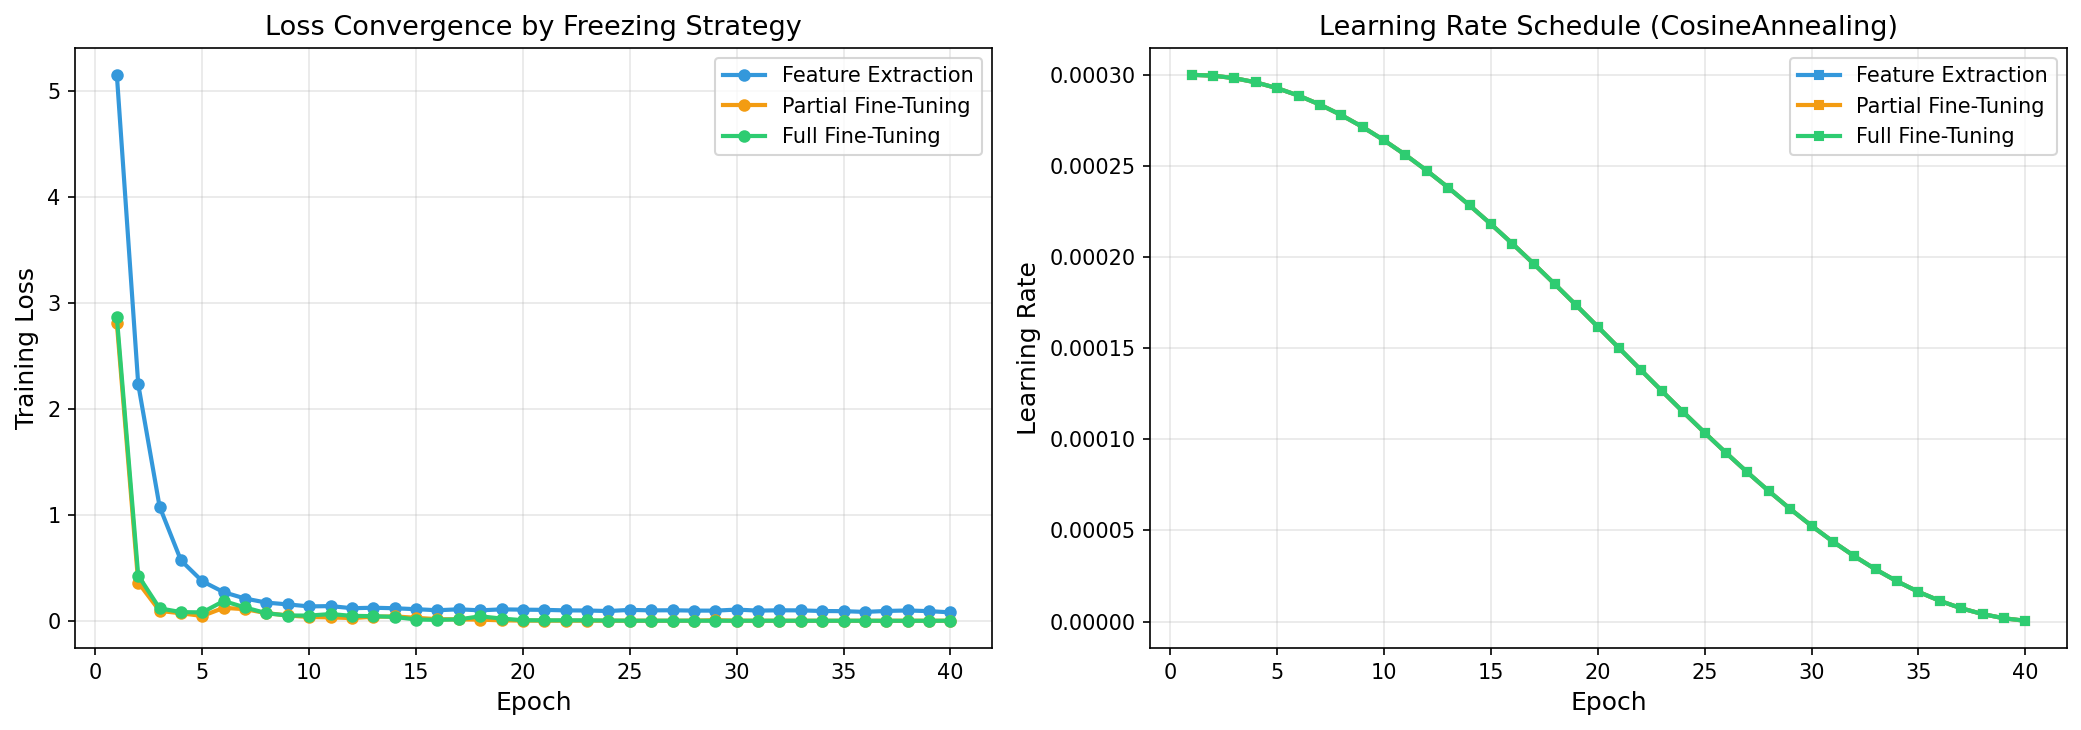
\includegraphics[width=\linewidth]{results/ablation_loss_curves.png}
  \caption{Courbes de perte pendant l'entraînement pour les trois stratégies de gel. Le gel total du backbone (Feature Extraction) atteint un plancher bien supérieur aux deux autres stratégies.}
  \label{fig:ablation_loss}
\end{figure}

Les résultats du tableau \ref{tab:ablation} et des courbes de figure \ref{fig:ablation_loss} montrent clairement que le gel total du backbone est catastrophique pour le Re-ID : les features ImageNet ne sont pas adaptées à la discrimination fine d'identités, et les 1,54M de paramètres entraînables (BN-Neck + classifieur) sont insuffisants pour surmonter ce déficit. Le fine-tuning partiel récupère l'essentiel de la performance ($+76$ pp par rapport au gel total) en libérant les couches hautes du réseau. Le fine-tuning complet apporte un gain supplémentaire de $+1,93$ pp en Rank-1 et $+4,22$ pp en mAP, au prix de $+6,7$ min d'entraînement -- un compromis favorable étant donné la disponibilité d'un GPU.

\subsection{WP5 : Comparaison architecturale ResNet-50 vs ViT}

\begin{table}[t]
\centering
\caption{Comparaison CNN/Transformer sur Market-1501. La latence est mesurée par image sur GPU.}
\label{tab:arch_comparison}
\resizebox{\linewidth}{!}{%
\begin{tabular}{lcc}
\toprule
Métrique & ResNet-50 & ViT-Base/16 \\
\midrule
Paramètres & 25,1M & 86,4M \\
FLOPs & 4,05 G & 6,46 G \\
Latence (ms/img) & 13,0 $\pm$ 0,6 & 10,7 $\pm$ 0,6 \\
Résolution & $256\times128$ & $224\times224$ \\
Dim. embedding & 2048 & 768 \\
\midrule
Rank-1 (\%) & 84,41 & \textbf{88,63} \\
mAP (\%) & 64,47 & \textbf{73,84} \\
Temps d'entraînement & $\sim$40 min & 47,9 min \\
\bottomrule
\end{tabular}}
\end{table}

\begin{figure}[t]
  \centering
  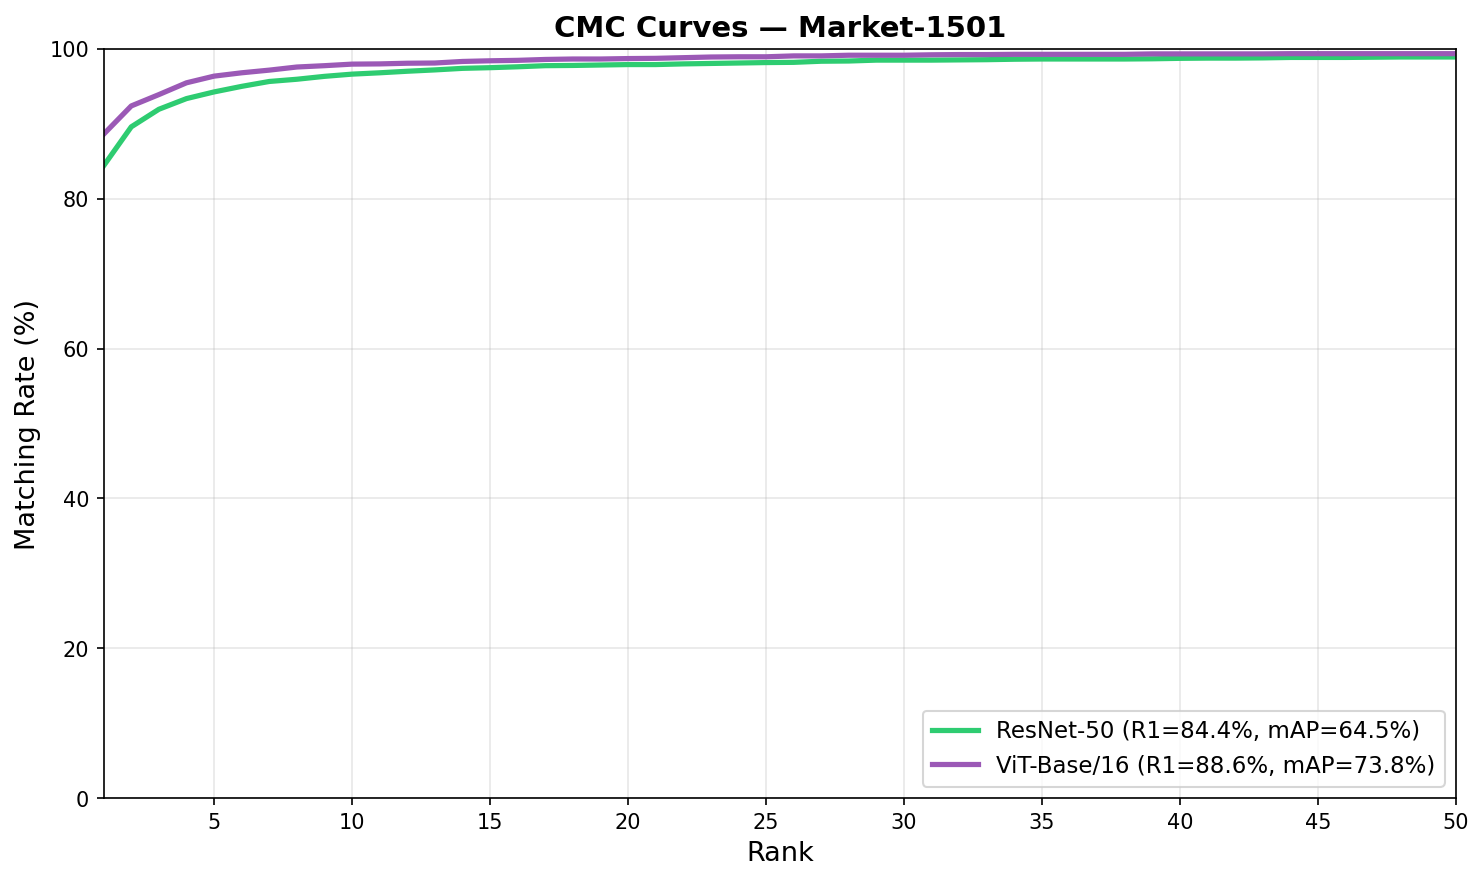
\includegraphics[width=\linewidth]{results/architecture_cmc_curves.png}
  \caption{Courbes CMC pour ResNet-50 et ViT-Base/16 sur Market-1501. ViT domaine à tous les rangs.}
  \label{fig:cmc_curves}
\end{figure}

Comme le montrent le tableau \ref{tab:arch_comparison} et la figure \ref{fig:cmc_curves}, ViT-Base/16 surpasse ResNet-50 sur tous les critères de qualité Re-ID : Rank-1 $+4,2$ pp, Rank-5 $+2,1$ pp, mAP $+9,4$ pp. Paradoxalement, ViT est plus rapide à l'inférence (10,7\,ms vs 13,0\,ms), car la convolution large du réseau est remplacée par des opérations matrice/vecteur efficacement parallélisables sur GPU. En revanche, ViT est 3,45$\times$ plus volumineux (86,4M vs 25,1M paramètres) et nécessite $\sim$20\,\% de temps d'entraînement supplémentaire. L'attention globale du Transformer lui permet de capturer des relations entre parties du corps spatialement distantes, ce qui se traduit par une meilleure séparation inter-classe dans l'espace d'embedding.

\subsection{WP6 : Adaptation de domaine}

\paragraph{Gap de domaine.}
Avant tout fine-tuning, nous mesurons le gap entre Market-1501 (source) et le dataset personnel (cible) à l'aide de la distance centraîde ($d_c = 0{,}603$), la similarité cosinus entre les centroids ($0{,}077$), et la MMD linéaire ($0{,}367$). Ces indicateurs confirment un décalage significatif entre les deux domaines, bien que les embeddings pré-entraînés se généralisent partiellement.

\paragraph{Résultats.}
\begin{table}[t]
\centering
\caption{Résultats d'adaptation de domaine (dataset cible : personnel). La mAP est la métrique principale en raison d'un artéfact d'évaluation sur un petit dataset (voir texte). Les Rank-1 et mAP du modèle source sont mesurés sur Market-1501.}
\label{tab:domain_adaptation}
\begin{tabular}{lcc}
\toprule
Expérience & Rank-1 & mAP \\
\midrule
Modèle source (Market-1501)  & 84,41 & 64,47 \\
Zero-Shot $\to$ Cible            & 100,00$^*$ & 78,27 \\
Transfer Learning $\to$ Cible    & 100,00$^*$ & \textbf{89,93} \\
\bottomrule
\end{tabular}
\vspace{2pt}
\footnotesize{$^*$ Rank-1 saturé : les images requêtes étant incluses dans la galerie, la correspondance exacte (sim. = 1) est toujours retournée en première position. La mAP (qui penalise le rang des \textit{autres} correspondances correctes) est plus représentative.}
\end{table}

\begin{figure}[t]
  \centering
  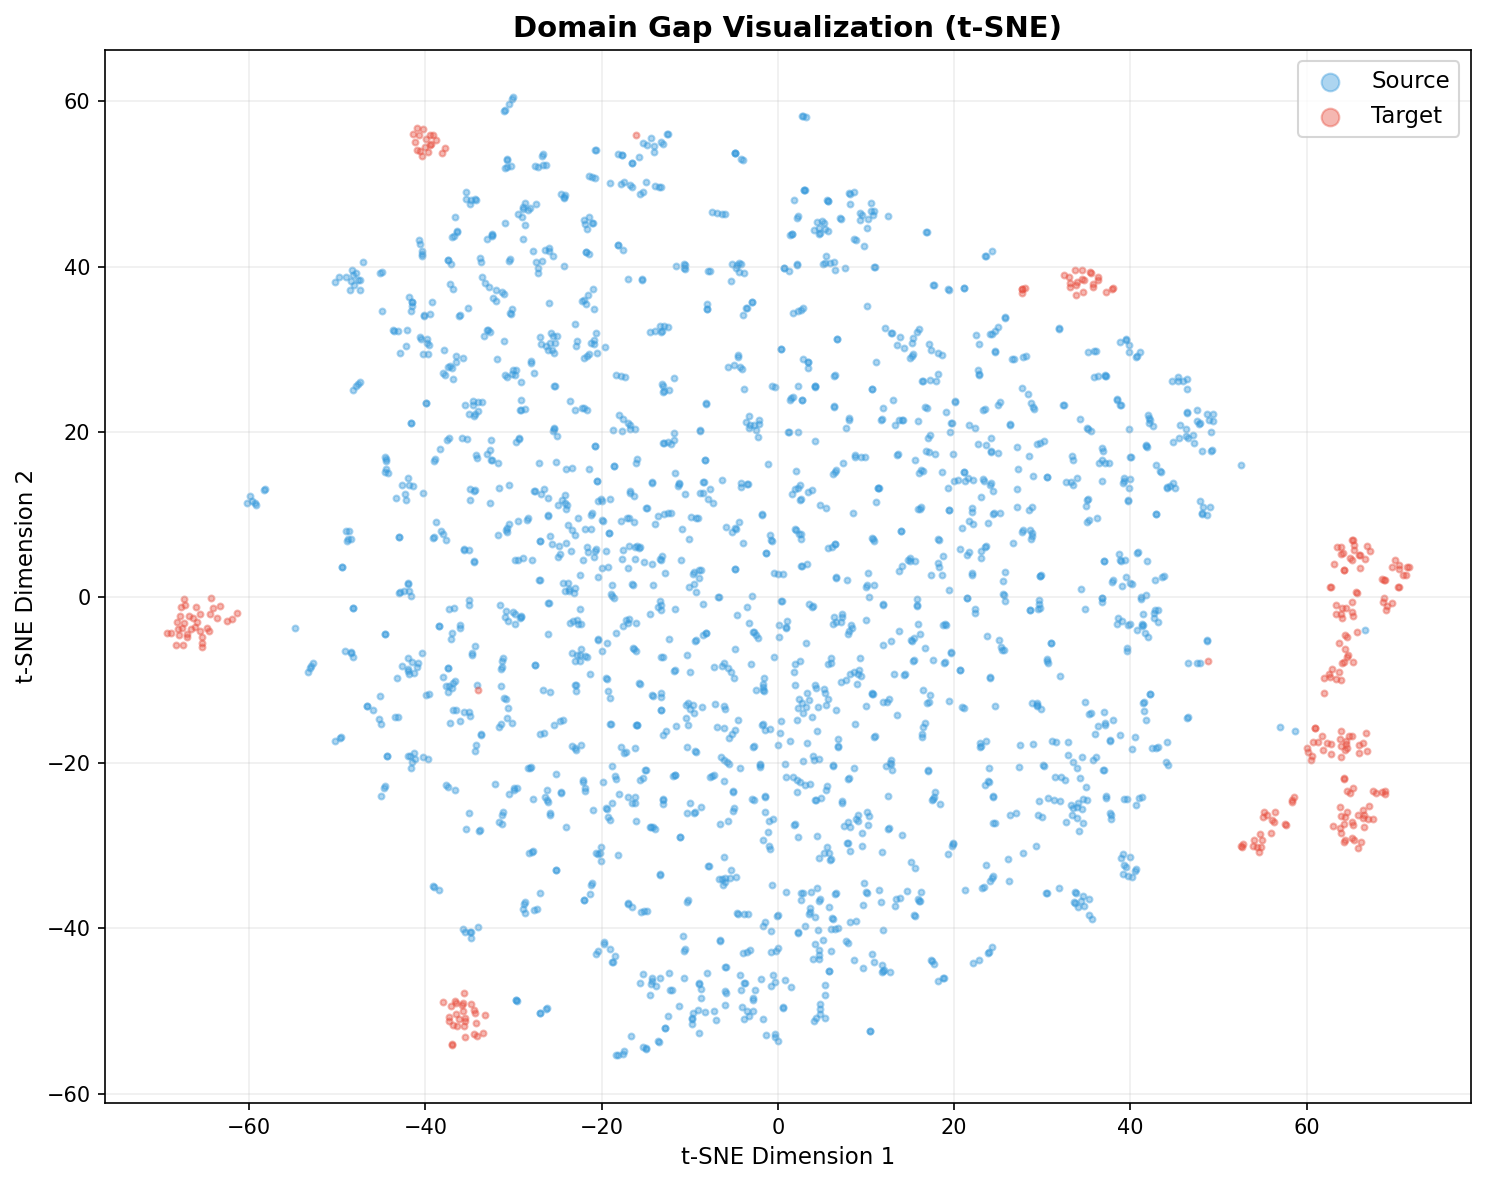
\includegraphics[width=\linewidth]{results/domain_gap_before_after.png}
  \caption{Visualisation t-SNE du gap de domaine avant et après adaptation. Après transfer learning, les embeddings du domaine cible s'organisent en clusters d'identité plus cohérents.}
  \label{fig:domain_gap}
\end{figure}

Le transfer learning (gel partiel, lr=$5 \times 10^{-5}$, 20 époques, 131 images) améliore la mAP de $+11,7$ pp (78,27 $\to$ 89,93\,\%). Cela démontre qu'un fine-tuning ciblé sur très peu de données (131 images) suffit à améliorer sensiblement la discrimination d'identité dans le domaine cible, même à partir d'un modèle entraîné sur un domaine différent.

\subsection{WP7 : Clustering d'albums}

\begin{table}[t]
\centering
\caption{Résultats du clustering DBSCAN ($\varepsilon = 0{,}18$) pour l'indexation automatique d'albums.}
\label{tab:clustering}
\resizebox{\columnwidth}{!}{
\begin{tabular}{lccc}
\toprule
Dataset & Pureté & Clusters & Imgs/cluster (moy.) \\
\midrule
Market-1501     & 88,95\,\% & 533 & 13,75 \\
Dataset personnel & \textbf{94,80\,\%} & \multicolumn{2}{c}{(eps optimal $\varepsilon \approx 0{,}15$)} \\
\bottomrule
\end{tabular}
}
\end{table}

La figure \ref{fig:domain_gap} (à gauche, identités source) illustre qualitativement la structuration des embeddings en clusters. DBSCAN est fortement sensible au seuil $\varepsilon$ : pour $\varepsilon \leq 0{,}15$, le nombre de clusters explose (plus de 500 pour Market-1501) fragmentant les identités ; pour $\varepsilon \geq 0{,}35$, l'effet de chaînage fusionne des identités distinctes en un seul mega-cluster (9 albums pour Market-1501 dont un de 12,804 images). Le pic de NMI et d'ARI, visible sur l'analyse de sensibilité, se situe à $\varepsilon \approx 0{,}2$ pour Market-1501 et $\varepsilon \approx 0{,}15$ pour le dataset personnel.

La pureté de 88,95\,\% sur Market-1501 (533 clusters, 13,75 images/cluster en moyenne, 191 images pour le plus grand) démontre que les embeddings ResNet-50 capturent efficacement l'identité plutôt que l'apparence brute -- le système gère les changements de pose et de caméra. Sur le dataset personnel (262 images, identités connues), la pureté atteint 94,80\,\%, confirmant la robustesse des features appris sur Market-1501 à un domaine différent.

\section{Conclusions}
\label{sec:conclusion}

Ce travail présente une étude systématique de la chaîne complète de ré-identification de personnes, de la construction du jeu de données à l'indexation d'albums sans supervision.

\paragraph{Synthèse des résultats.}
(i) Les descripteurs classiques (HOG, couleur, SIFT) sont largement insuffisants pour le Re-ID (Rank-1 $< 2$\,\%), tandis que le re-ranking k-réciproque apporte un gain significatif de mAP ($+9,5$ pp) sur les embeddings profonds. (ii) L'ablation sur les stratégies de gel confirme que le gel total du backbone empeche toute adaptation discriminante: seul le fine-tuning complet (ou partiel au minimum) permet d'obtenir des performances viables. (iii) ViT-Base/16 surpasse ResNet-50 en qualié de classement (Rank-1 88,63\,\% vs 84,41\,\%) tout en étant legèrement plus rapide à l'inférence, malgré un budget paramétrique 3,45$\times$ plus élevé. (iv) Le transfer learning sur seulement 131~images du domaine cible améliore la mAP de 78,27\,\% à 89,93\,\%, illustrant la capacité du fine-tuning à combler rapidement un gap de domaine. (v) DBSCAN sur embeddings ResNet-50 permet une indexation automatique avec 88,95\,\% de pureté sur Market-1501 et 94,80\,\% sur le dataset personnel.

\paragraph{Perspectives.}
Plusieurs améliorations sont envisageables: (a) élargir le dataset personnel (actuellement 262 images) pour rendre l'évaluation de l'adaptation de domaine plus robuste et corriger l'artéfact d'évaluation query/galerie~; (b) explorer des méthodes d'adaptation de domaine sans supervision (UDA), évitant la nécessité d'annotations manuelles dans le domaine cible; (c) tester des architectures Re-ID plus spécialisées (TransReID~\cite{he2021transreid}, AGW~\cite{ye2021deep}) avec des mécanismes d'attention sur les parties du corps~; (d) intégrer un pipeline de clustering itératif avec pseudo-étiquettes pour un entraînement semi-supervisé dans le domaine cible.

{
    \small
    \bibliographystyle{ieeenat_fullname}
    \bibliography{main}
}
\end{document}
